\documentclass[12pt]{report}
\usepackage{graphicx}
\graphicspath{{Images/}}
\usepackage{textcomp} %for the copywrite symbol
\linespread{1.6} %sets lines to 1.5 spacing.  1.6 would be double spaced
\usepackage[margin=1.0in]{geometry}
\usepackage[semicolon,round,sort&compress,sectionbib,numbers]{natbib}  
\usepackage{chapterbib}  
\usepackage{amsmath}
\usepackage{subcaption}


\usepackage{hyperref} %make stuff clickable
\hypersetup{
	colorlinks,
	citecolor=black,
	filecolor=black,
	linkcolor=black,
	urlcolor=black
}


\usepackage{physics}  %for bras and kets!
\newcommand{\angstrom}{\mbox{\normalfont\AA }} %makes \angstrom do its thing!
 
\begin{document}





\begin{titlepage}
    \begin{center}
        \vspace*{1cm}
        \huge
        {Density Functional Theory Techniques for Electron Energy Loss Analysis of Lithium Materials}
        
       
        
        
        
        \vspace{1.5cm}
        
        \large
        {Quentin Stoyel, Mining and Materials Engineering, McGill University, Montreal}\\
        
        {November 2018}
        
        
       \normalsize
       A thesis submitted to McGill University in partial fulfillment of the requirements of the degree of Masters of Science
        
		\vfill
        
		\includegraphics*[scale=1]{McGill_logo.png}
        
        {\textcopyright Quentin Stoyel 2018}
    \end{center}

\end{titlepage}










\chapter*{Abstract}
\renewcommand{\thepage}{\roman{page}}% Roman numerals for page counter

\addcontentsline{toc}{section}{Abstract}

A new method of calculating the magnitude of the core hole screening in the case of lithium materials is developed and implemented for the accurate simulation of Energy Loss Near Edge Structure (ELNES).  ELNES is calculated for Li, $\mathrm{Li_2O}$, and LiF with marked improvements in agreement between calculation and experiment, as well as superior quantitative and predictive abilities.   The technique uses linear response theory to relate the electron density to the core hole shielding contribution from the valence electrons in a molecule.  This contribution is then implemented via a non integer core hole in final state rule calculations. 
\\
Abstract in French too

\chapter*{Acknowledgements}
\addcontentsline{toc}{section}{Acknowledgements}
To all those useful folks

\chapter*{Contribution to Original Knowledge}
\addcontentsline{toc}{section}{Contribution to Original Knowledge}
A new method of simulating ELNES with a focus on Lithium materials was developed.  Density functional theory results are used to simulate Electron energy loss fine structure.  The core hole approximation ex



\tableofcontents

\chapter{Introduction}
\renewcommand{\thepage}{\arabic{page}}% Arabic numerals for page counter
\setcounter{page}{1}% sets page number


%Batteries are important

%Use EM to analyze them

%In particular EELS is good

%Want simulations, use DFT
 
%Want better simulations improve core hole method
\setcitestyle{numbers,open={[},close={]}}

The study of lithium materials has become increasingly relevant over the years.  In particular, the field has been driven by the need to develop improved battery materials.  This drive has come from an array of fields, amongst others, electric vehicles and portable electronics desiring longer lifetimes and faster charging.  All aspects of batteries are currently being improved including capacity, charge density, and charge/discharge rates.  As well as performance, other features such as safety and the ability to reuse or recycle battery materials are also growing fields.  \\
In the realm of performance, lithium ion batteries offer a wide range of advantages.  Lithium is the third element on the periodic table and consequently offers very high charge densities.  This allows for batteries to become smaller and lighter without sacrificing lifetime.  Additionally, lithium's lightweight nature make it highly mobile which is an attractive feature for increasing maximal discharge rate.  Finally, as an alkali earth metal with a single weakly bound valence electron, lithium is highly electropositive  which allows lithium ion batteries to achieve higher operating voltages than alternatives such as nickle-cadmium or lead-acid batteries.  These potential performance advantages are illustrated in Fig \ref{ragone}.
\\

\begin{figure}
	\centering
	\includegraphics[scale=0.3]{ragone_plot}
	\caption{Plot illustrating the the power and energy densities achievable by three types of battery, as well as the minimum requirements for various types of electric vehicle, including hybrid electric vehicles (HEV), plug in hybrids (light vehicle). From \cite{etacheri_challenges_2011} }
	\label{ragone}
	
\end{figure}
The pursuit of developing new and improved battery materials has shifted the focus of analysis towards studying the microstructure of materials. The ability to identify crystal structure and composition has become an essential element to understanding and tailoring material properties.  On this front, electron microscopy has become a central technique to this effort  \cite{inkson_2_2016}.  Rapidly improving technology, the possibility of atomic level resolution, coupled with the increasing accessibility have made electron microscopy one of the most prevalent techniques for studying nanoscale features in materials.  Here, however lithium is at odds with the method.  Novel battery materials are increasingly intricate and lithium's lightness and easy to ionize nature make it particularly sensitive to electron beams, complicating analysis.  Additionally, as the third element, it lies outside the ranges of many conventional theories.  These properties make electron energy loss spectroscopy (EELS), a low dosage technique that is well suited for light elements such as lithium, attractive for battery material analysis   \cite{Egerton}.  However, EELS results have been historically qualitative and require strong theoretical support to be analyzed.  The theoretical support is all the more essential in dealing with novel lithium materials that have limited sample life.   
\\
The theoretical support for EELS can come from a number of methods, however, the most prevalent of these are based in density functional theory (DFT), a first principles approach that requires only the locations of atoms in a crystal to determine material properties \cite{ks_1965}.  Here too, results have been limited to qualitative findings, further complicated by lithium's lightweight nature which also poses challenges to theoretical approaches.  The work performed in this thesis was to address some of the issues facing DFT methods concerning EELS of lithium.  In particular, an improved method of calculating electron screening was implemented to improve the core hole approximation used to handle excitonic effects.  
\\

The outline of this thesis is as follows: in Chapter 2 we will begin with an overview of EELS, DFT and theoretical EELS calculations.  Chapter 3 will describe the improved method developed in this work, and Chapter 4 will apply the method to a number of lithium materials.  Chapter 5 will conclude the results and address future work.





\chapter{Literature Review}\label{literature_review}

%What is eels?
%Sample experimental setup
%Sample spectra
%Signal types
%usages
%pros, cons/ STEM TEM
\setcitestyle{numbers,open={[},close={]}}


The focus of this work lies on theoretical calculations from first principles, designed to provide information on materials without the need for experiment.  However, in order to verify new techniques, they must be confirmed with experiment.  To this end, this chapter will commence with an overview of experimental electron microscopy and  energy loss spectroscopy(EELS) before investigating how it is performed in the  structure of density functional theory (DFT). We will conclude with a review of the various methods used to calculate EELS theoretically.  The particularities of lithium materials will be discussed at each step of this process.  
 
\section{Electron Energy Loss Spectroscopy}

\subsection{Background}
Materials are becoming increasingly refined with properties requiring characterization of nano scale features to unlock their full potentials \cite{goldstein_electron_2003}.  At these length scales, even state of the art light microscopes lack the resolution to discern these features \cite{rust_sub-diffraction-limit_2006}.  This limitation is due to the fact that nano scale features fall well below the diffraction limit of light microscopes \cite{hecht}: 

\begin{equation}
	d = \frac{\lambda}{2n\textrm{ sin}(\theta)}
\end{equation}

Where n is the refractive index and d is the smallest distance between 2 discernible objects. For optical light ($\lambda$ = 400-800nm), it is impossible to routinely achieve the desired resolution ($\sim$ 1-50 nm) for characterization \cite{rust_sub-diffraction-limit_2006}.  Electrons however have a wavelength dictated by \cite{goldstein_electron_2003}: 
\begin{equation}
 \lambda = \frac{h}{\sqrt{2 m_0 e E}}
\end{equation}
Where $h$ is planck's constant, $m_0$, $e$ and $E$ are the rest mass, charge and energy of an electron.  In an electron microscope, electrons are accelerated to energies on the order of 1-100 keV giving them wavelengths in the range from 1-100 pm ($1\mathrm{pm}=10^{-12}$m).  Electron microscopes can therefore achieve a far lower theoretical diffraction limit  and are currently limited by the technological constraints of the electron  lenses \cite{goldstein_electron_2003}.  Because of this high resolution, electron microscopes have become a key part of investigating material microstructure \cite{inkson_2_2016}.  This dramatic increase in resolution compared to alternative methods is illustrated in Fig \ref{method_scales}. 
\begin{figure}
	\centering
	\includegraphics[scale=0.3]{method_scales}
	\caption{Resolution achievable by various techniques including Transmission and Scanning electron microscopy (TEM/SEM) and light microscopy, on a log-log scale.  Taken from Inkson, 2016 \cite{inkson_2_2016}}.
	\label{method_scales}
	
\end{figure}

In addition to the ability to image samples with high resolution, electron microscopy generates a large number of different and useful signals which can be used for both to characterize samples as well as imaging them, see Fig \ref{specimen_emmisions} \cite{williams_transmission_2008}.  A full discussion of the various techniques electron microscopes used to investigate each of these accessible signal types is beyond the scope of this work and has been well documented elsewhere \cite{goldstein_electron_2003,Egerton,williams_transmission_2008,reimer_electron_1998}.  Instead, we will focus on the relevant technique, electron energy loss spectroscopy (EELS).  EELS is an electron microscopy technique that analyzes the transmitted inelastically scattered electrons, Fig \ref{specimen_emmisions}\cite{Egerton}.  It is mainly an analytic technique, however it is also possible to perform imaging with EELS \cite{varela_stem-eels_2012}.  EELS consists of collecting electrons that have passed entirely through the sample and binning them according to how much energy each one has lost, resulting in a spectrum such as in Fig \ref{EELS_spectra}.  The mechanism of energy loss for the beam electrons is by exciting the samples electrons in a number of ways, which is reflected by the multiple different features in the spectrum \cite{Egerton}. The main features in EELS spectra are: 
\begin{figure}
	\centering
	\includegraphics[scale=0.3]{specimen_emmisions.png}
	\caption{The numerous types of signals emitted when an electron beam encounters a sample in a TEM/STEM.   Redrawn from Williams and Carter \cite{williams_transmission_2008}.  }
	\label{specimen_emmisions}
\end{figure}

\begin{figure}
	\centering
	\includegraphics[scale=0.3]{EELS_spectra.png}
	\caption{Sample EELS spectra identifying the main features, the zero loss peak, plasmon peak and ionization edges wwith fine structure.   The intensities are on a log scale, and span approximately 6 orders of magnitude between the zero loss and the ionization edges.  }
	\label{EELS_spectra}
\end{figure}

\begin{itemize}
	\item \textbf{Zero Loss Peak:} The majority of the electrons in EELS pass through the specimen without experiencing an inelastic interaction, and retain their initial energy.  The width of this peak defines the resolution of the spectrum and is due to energy spreading as the beam passes through the electron lenses \cite{colliex_illustrated_1985}.  For thin samples, zero loss peak is also the most intense feature on a spectrum \cite{Egerton}.  
	
	\item \textbf{Plasmon Peak:}  The electron beam can excite multiple atoms in the solid collectively, creating a wavelike oscillation in electron cloud of the solid \cite{Egerton}.  These ae called plasmon excitations and result in a peak appearing between 5-30eV \cite{Egerton}.  The shape and intensity of the peak is dependent on the bond strength in the material and can be used to probe properties such as thickness and surface topology \cite{malis_eels_1988,nelayah_mapping_2007}. 
	
	\item \textbf{Ionization Edges:} Beam electrons can also excite core electrons in the sample to the conduction band.  As an atom's core states are in general isolated from its surroundings, the ``edges" for each element will occur at specific energy locations, independent of sample, analogous to characteristic x-rays \cite{Egerton}. These can be used to determine sample composition \cite{Egerton}.  
	
	\item  \textbf{Background:} Beam electrons can excite loosely bound electrons close to the Fermi level into the unoccupied conduction band.  Due to the large number of possible transitions and the fact that high energy events are less favourable, this results in a smoothly decaying background \cite{Egerton}.

	
\end{itemize}

%The probability of each event depends on a number of factors.   Foremost amongst these is that the higher the energy of an event, the less likely it is to occur (CHECK!!!). This is highly dramatic as can be seen by the N orders of magnitude required to show all of these features.  

Another key factor that needs consideration, is that in order for meaningful data to be extracted from a spectra, the number of electrons that experience multiple inelastic events must be minimized \cite{Egerton}.  If not, duplicate plasmon peaks will appear in the spectra, and because of their relatively high intensity, the weaker ionization edges will become drowned out by the background, see Fig \ref{multiple_plasmons}. As well, any electron that experiences an ionization event will likely also experience some form of plasmon interaction, further smearing any ionization edges in thicker samples.  

\begin{figure}
	\centering
	\includegraphics[scale=0.2]{multiple_plasmons.png}
	\caption{Two spectra demonstrating the importance of thin samples and single scattering events. In the thicker sample, the majority of beam electrons experience one or multiple plasmon excitations, resulting in multiple evenly spaced plasmon peaks with larger intensity than the zero loss.  The higher background from the plasmon peaks and the thicker sample drown out any structure due to ionization edges \cite{Egerton}. Image taken from Egerton, 2011 \cite{Egerton}}
	\label{multiple_plasmons}
\end{figure}



\subsubsection{Near Edge Structure}
Unlike x-ray edges in EDS which have distinct, simple shapes, higher energy resolution in EELS reveals additional features in the ionization edges extending up 50 eV beyond the onset of the edge \cite{Egerton}.   These features are a reflection of the unoccupied states in the conduction band that represent the final states of sample electrons excited by the beam.  The band structure of the conduction band is largely dependent on the local bonds of the atom in question.  Because of this, ELNES can be used to investigate the local environment of each element.  This can be used to distinguish different crystal structures of the same element such as carbon in graphite vs diamond, see Fig \ref{carbon-k-edge} \cite{hamon_elnes_2004}.  ELNES is also sensitive to impurities that would effect the band structure.  

\begin{figure}
	\centering
	\includegraphics[scale=0.5]{Carbon_k_edges}
	\caption{Carbon K edge taken at 30keV at McGill. The different crystal structures (amorphous, diamond and carbon nanotube) result in distinctly different ELNES which can be used for identification.   }
	\label{carbon-k-edge}
\end{figure}


\subsection{EELS in Experiment}

In order to collect EELS spectra, electrons must pass entirely through the sample, making EELS a technique for transmission electron microscopes (TEM's)\cite{Egerton}. In order to collect these transmitted electrons, a magnetic field prism is placed below the specimen and redirects the electrons into a detector, Fig \ref{prism}.  Inside the magnetic prism, there is a $\mathrm{\textbf{B}}$ field perpendicular to the beam direction and the transmitted electrons are exposed to a Lorentz force: 


\begin{equation}
	\textbf{F}_B = q (\textbf{v} \times \textbf{B})
\end{equation}

As the force varies according to the velocity of the electrons, the magnetic prism  separates the electrons according to their energy: 

\begin{gather}
\textbf{F}_B = e (\textbf{v} \times \textbf{B}) =  \frac{m \textbf{v}^2}{\textbf{r}} = \textbf{F}_c \\
 r =  \frac{mv}{eB} = \frac{\sqrt{2mE}}{eB}
\end{gather}

\begin{figure}
 \centering
 \includegraphics[scale=0.4]{Expt_setup.png}
 \caption{Experimental EELS setup, with the various magnetic lenses depicted in blue.  }
 \label{prism}
 
\end{figure}

Where e is the charge of an electron and E is the energy of each electron after passing through the sample.  By mapping each location on the detector to a corresponding energy loss value the final spectra are obtained. In order to produce images, the beam is rastered over the sample and the intensities of a specific energy loss value are used to create an image. 

\subsubsection{TEM vs SEM EELS}
There are two main types of electron microscopy, scanning and transmission (SEM and TEM).  TEM typically operates with beam energies between 100-300 keV while SEM performs between 1-30 keV.  Each method has their own set of advantages.  TEM's operate on thin samples resulting in a minimal interaction volume, resulting in far higher energy resolution and have the ability to image individual atoms. SEM's scan the surfaces of samples and can operate on bulk specimens.  SEM is also dramatically more economical and flexible of a technique.   EELS has been conventionally performed in TEM's as it requires the beam to pass through the sample. Recent advances however have allowed EELS to be performed in an SEM.   EELS in an SEM offers the distinct advantage over TEM EELS for lithium materials as it allows operation at 30keV which minimizes the beam damage.  It is also dramatically more economical.   

\subsubsection{Lithium in EELS}
Lithium materials present a number of challenges to EELS analysis.  As the lightest alkali metal it is almost always ionized and highly mobile. Additionally, lithium ion battery materials are in general insulators with band gaps of varying sizes. These features make lithium materials highly sensitive to electron beam damage.  This damage results from the charge buildup when an electron beam passes through a sample.  In electron conductive samples (eg. metals), this charge can be dissipated to a certain extent, however in materials with a band gap (eg. insulators, battery cathodes), this charge can displace the charged and mobile lithium ions and break down the crystal structure.  Lithium's high mobility also make them vulnerable to knock on damage.  This effect occurs when an electron interacts inelastically with an atom's nucleus and transfers sufficient energy to it to displace it from its lattice site.  Lithium is particularly vulnerable to this interaction because its lightweight and high mobility, meaning that it requires only a small amount of energy ($ \sim 1-5$eV) to displace it through a crystal.\\  
Lithium's only ionization edge is its K-edge is located at $\mathrm{\sim}$55eV, at the boundary of what is considered reasonable for analysis.  The low edge places it close to the plasmon decay complicating background subtraction.  This energy range also often results in overlap between the lithium K-edge and the $\mathrm{M_{2 / 3}}$ and $\mathrm{M_4}$ edges of transition metals. In particular the edges of Mn, Fe and Ni, all fall between 40-70eV.  As these elements are key components to cathode materials, they can require further steps for analysis to be possible.



\subsection{Preprocessing}

There are two key steps to be performed upon acquiring an ELNES spectra before it can be used for meaningful conclusions, background subtraction and deconvolution. 

\subsubsection{Background Subtraction} \label{bg_section}
The smooth decaying background in EELS spectra needs to be removed in order for meaningful comparison and measurements to be made on ELNES.  However, the EELS background does not decay at a fixed rate and changes based on the presence of edges and with energy \cite{new_bg}. Consequently, it is not currently possible to fit remove a single function to an entire spectrum.  Instead, the method of choice relies on fitting to a window directly before an ionization edge and refitting for each edge as needed.  The most prevalent function used for this purpose is a power law decay \cite{Egerton}: 

\begin{equation}
	I_{bg} = AE^{-r}
\end{equation}

Where E is the energy loss and A and r are fitting factors.  This method has limitations due to different regions of the spectra decaying at different rates which means a fit must be performed for every analysis \cite{verbeeck_model_2004, egerton_inelastic_1975}.  A downside of this method is the final results dependence on the size and location of the fitting window on the final output, see Fig \ref{bg_removal}.  This instability has resulted in a number of alternate models being proposed for specific cases, however, the power law method remains the most prevalent \cite{verbeeck_model_2004, riedl_extraction_2006}.  

\begin{figure}
	\centering
	\begin{subfigure}{0.45\textwidth}
		\includegraphics[scale=0.5]{full_bg.png} 
		\caption{}
		\label{full_bg}
	\end{subfigure}
	\hfill
	
	\begin{subfigure}{0.45\textwidth}
		\includegraphics[scale=0.5]{good_window.png} 
		\caption{}
		\label{good_window}
	\end{subfigure}
	\begin{subfigure}{0.45\textwidth}
		\includegraphics[scale=0.5]{bad_window.png} 
		\caption{}
		\label{bad_window}
	\end{subfigure}
	\caption{Results of power law background removal from raw spectrum (a) of metallic lithium K edge, using an appropriate (b)and inappropriate (c) window choice.}
	\label{bg_removal}
\end{figure}

\subsubsection{Deconvolution} \label{deconvolution}
Despite drastic improvements, there is still a degree of energy spread on beam electrons, typically in the range of $\sim$0.5-3eV.  This energy spread results in the observed ELNES on a spectra to be a result of a convolution between the 'actual' ELNES and the zero loss peak.  Additionally, the probability of an electron undergoing plural scattering (scattering inelastically more than once in the specimen) must also be accounted for, as the low loss region of the spectrum is also convoluted into the output spectra.  Plural scattering can best be seen in thicker samples where it results in the presence of multiple plasmon peaks, although it is present on the entire spectrum.  In order to recover the single scattering spectrum, the output must undergo deconvolution.  A number of techniques exist for this purpose.   Fourier techniques rely on describing the signal as a number of convolutions:

\begin{equation}
 	J(E) = Z(E))\ast[\delta(E) + \frac{S(E)}{I_0} +  \frac{S(E) \ast S(E)}{2! I_0}   + ...]
\end{equation}



Where J(E) is the obtained spectra, Z(E) is the zero loss peak, S(E) is the single scattering spectra, and I$_0$ is the integrated intensity of the zero loss.  The double scattering term is the convolution of the two single scattering terms, weighted by the decreased probability according to Poisson statistics.   Taking a Fourier transform of this turns all of the convolutions into products: 

\begin{equation}
	j(\nu) = z(\nu) \left(1+\frac{s(\nu)}{I_0}+   \frac{s^2(\nu)}{2! I_0}+ \frac{s^3(\nu)}{3! I_0} + ...\right)
	\label{fourier_spectra}
\end{equation} 

Which can in turn be collapsed into an exponential:

\begin{equation}
	j(\nu) = z(\nu)\mathrm{exp}[s(\nu)/I_0]
\end{equation}

This equation can then be solved for $s(\nu)$ and reverse Fourier transformed to obtain the single scattering spectra.  In order to avoid amplifying the noise in the original spectra, which is represented by high frequency terms in Fourier space, the result must be broadened by a modifier to minimize these terms.  Thus, deconvolution can only improve the energy resolution of a spectra to a certain extent.  

More recently, Bayesian methods have found success as well, in particular the Richardson-Lucy technique \cite{richardson_lucy}. This technique is based on iterative methods initially developed in astronomy and used for the deconvolution of images, including some from the Hubble space telescope \cite{hubble}.  From the same starting point, the convolution of the ideal spectra with the low loss, or point spread function:

\begin{equation}
J(E) = R(E)\ast S(E)
\end{equation}

As an EELS spectra is inherently pixilated by the CCD, at each pixel we can apply Poisson statistics to define the probability of obtaining the observed number of counts (N) \cite{richardson_lucy}:  

\begin{equation}
	P (N/N_m) = \frac{e^{-N_m}N^N_m}{N!}
\end{equation}

By iteratively varying N$_m$ and maximizing the probability, the deconvoluted spectra can be obtained.  Similar to Fourier methods however, the noise on the spectra increases with more iterations, in order to conserve information.   


\subsection{Other Experimental Techniques}
EELS is by no means the only experimental technique available for the analysis of material microstructure, nor is it even the only electron microscopy technique available for the task. Other prevalent techniques include x-ray based analysis such as x ray absorption spectroscopy and energy dispersive spectroscopy.  We will take a moment to briefly describe these methods.

\subsubsection{X Ray Absorption Spectroscopy (XAS)}
XAS operates on a similar principle to EELS.  Instead of probing the sample with an electron probe, a beam of x-rays is directed through the sample and the resulting energy losses in the output spectrum are binned as in EELS \cite{groot_high-resolution_2001}.  The difference in probe media does not effect the measured quantity which is the same as in EELS: the unoccupied density of states of the material \cite{groot_high-resolution_2001}.  Because of their similarities, parallels are often drawn between EELS and XAS when developing theories.  The largest benefit of XAS is it's superior energy resolution ($\sim$0.1 eV) when compared to EELS ($\sim$1 eV) allowing for more features in near edge structures to be identified\cite{Egerton, groot_high-resolution_2001}.  This benefit comes at a cost however, XAS needs to be performed in a synchrotron, making it far more costly and less accessible to perform than EELS


\subsubsection{Energy Dispersive Spectroscopy (EDS)}
EDS is another form of analytic spectroscopy performed in electron microscopy.   Unlike EELS and XAS which measure the unoccupied density of states, EDS measures the occupied DOS \cite{goldstein_electron_2003}.  Like EELS, EDS probes the sample with an electron beam, but then collects the emitted x-rays produced when the sample electrons return to their relaxed states following excitation.  These x-rays have the same characteristic energies as in EELS, but EDS lacks the resolution to distinguish fine structure.  As such, it is limited to providing composition information on samples.  EDS is however less strict on sample requirements as it does not require the thin samples needed by EELS and can therefore be used to analyze both bulk and microscale features in samples \cite{goldstein_electron_2003}.

\subsection{Lithium in EELS}
The focus of this work lies in application to lithium materials and a brief discussion of their experimental nature is in order. Lithium's lightweight, easily ionizable nature that make it ideal for battery applications come at the cost of making lithium remarkably sensitive to an electron beam. The highly energized charged beam of electrons used to analyze sample in a SEM/TEM inflicts a range of damage onto lithium samples including evaporation of lithium and collapse of crystal structures.  As such minimizing beam exposure is essential to performing measurements on lithium materials.  EELS is an effective means of reaching this target, as it is possible to obtain signal from the majority of ionization events and requires only a few seconds to obtain.  However, in EELS lithium presents a new challenge, the only ionization edge lies at $\sim$ 55 eV close to the background tail of the plasmon peak.  As a result, lithium EELS specimens must be made thin enough to minimize plural plasmon scattering or risk drowning out the relatively weak lithium k-edge features.  

A second range of features of lithium are its minimal interactions with x-rays.  As such a light element, lithium has a low fluorescence yield, producing a single x-ray per 10,000 ionization events.  Additionally, lithium's low Z number also results in a minimal cross section relative to interact with x-rays.  Consequently, lithium is essentially invisible to x-ray diffraction (XRD) techniques, and can only be detected on the most sensitive electron dispersive spectroscopy (EDS) systems.

These various features highlight impressive technological advances that have been necessary to even study lithium experimentally on this size scale.  They also demonstrate the need for strong theoretical support to interpret novel lithium results obtained in challenging situations.  





\section{Density Functional Theory}\label{dft_section}

%What is eels?
%Sample experimental setup
%Sample spectra
%Signal types
%usages
%pros, cons/ STEM TEM
\setcitestyle{numbers,open={[},close={]}}

 


Many of the results from EELS have non-intuitive interpretations, particularly in the case of ELNES which relies largely on qualitative comparisons between measured and database spectra.  Consequently, new materials and situations require a degree of theoretical support to analyze novel results.  This support often comes from ab initio calculations, amongst others density functional theory (DFT).  This section will describe the basis of DFT and its various implementations, as well as discuss the peculiarities of simulating lithium materials.

\subsection{Background}
DFT is an ab initio method that requires only atomic positions as input and is independent of experimental support.  By solving a modified version of the Schrodinger equation, it is possible to obtain the ground state energy of the system, and from there determine a range of other properties, including EELS spectra. This almost direct treatment of quantum mechanics make DFT one of the most accurate techniques, however, the quadratic to cubic scaling of the method, limit its applicability to small scale systems, Fig \ref{scaling}.  DFT's success and flexibility have resulted in the development of a large number (90+) of codes, both open source and commercial, and its place in a wide array of fields \cite{DFT_codes}.  

\begin{figure}
	\centering
	\includegraphics[scale=0.3]{method_scaling.png}
	\caption{Various methods available to compute material properties and their corresponding regions of use. }
	\label{scaling}
\end{figure}


\subsection{Formulation}

DFT relies on solving the multi-bodied form of the Schrodinger equation \cite{sholl_density_2009}.  Our aim is to obtain a solution for $\psi$ from which observable properties can be calculated:  

\begin{equation}
	\frac{-\hbar^2}{2} \sum_{i}^{N} \frac{\nabla^2 \psi_i}{m_i} + \sum_{i}^{N} V(\textbf{r}_i) \psi_i = E \psi
\end{equation}

In this case, we will consider the non-relativistic, spin independent, time independent case, although more in-depth derivations can be found elsewhere \cite{tddft}.  We will now apply the Born Oppenheimer approximation, and assume that the nuclei can be separated from the electrons and will act classically. The validity of this assumption stems from the fact that nuclei are a  over 1000 times more massive than electrons \cite{graff_direct_1980}.  The Born Oppenheimer approximation allows us to only solve for the $\psi$ of electrons:

\begin{equation}
	\bigg[\frac{-\hbar^2}{2m_e}\sum_{i}^{N} \nabla^2 +\sum_{i}^{N} V(\textbf{r}_i) + \sum_{i}^{N}\sum_{j <i}U(\textbf{r}_i,\textbf{r}_j) \bigg] \psi_i(\textbf{r}_i) = E \psi_i
\end{equation}

Where $m_e$ is the mass of an electron, N is the number of electrons, and $\textbf{r}_i$ is a position vector. The terms inside the square brackets are collectively know as the Hamiltonian and are respectively: the kinetic energy of all the electrons, the Coulomb interaction between the electrons and the nuclei, and the electron-electron Coulomb interaction  \cite{sholl_density_2009}. At this point, these equations are still too unwieldy to solve, depending on 3N variables (the position coordinates of each wavefunction), not to mention the many body problem lurking inside the double sum.  Facing this conundrum, we take advantage of the Hohenberg-Kohn Theorems which postulates \cite{hohenberg_inhomogeneous_1964}:
\begin{itemize}
	\item  The ground state \textit{energy} of the system is a unique functional of the ground state \textit{electron density}.
	\item The electron density that minimizes the overall energy corresponds to the real ground state density.  
\end{itemize}

By changing the variables being solved for to the \textit{density} and not wavefunctions, we can simplify the problem down to only three variables: the three coordinates of the density field.  The Hohenberg-Kohn theorems indicate that we can make everything a functional of electron density and that any density other than the groundstate will result in a higher energy in the system \cite{parr_density_1983}.  We now define the term functional, as an object that acts like a function, except takes other functions as input instead of variables, eg:

\begin{equation}
F[f(x)] = f(x)^2 
\end{equation}

 In the case at hand, the relevant functional is the energy which is a functional of the density: $E[n(\textbf{r})]$.  Using the Hohenberg-Kohn theorems, we can begin working towards a more manageable equation for energy by further breaking down the potentials and writing as functional of density: 
\begin{equation}
-\frac{\hbar}{2m_e} \sum_{i} \int \psi_i^* \nabla^2\psi_id^3r + \int V(\textbf{r})n(\textbf{r})d^3r + \frac{e^2}{2} \int \int \frac{n(\textbf{r})n(\textbf{r}')}{|r-r'|}d^3r d^3r' + E_{\mathrm{nuclei}} + E_{\mathrm{XC}} = E[\psi_i]
\end{equation}

Where the first term is the kinetic energy of the electrons, the second is the energy from the electron density-nuclei interaction with $V(\textbf{r})$ is the electric field created by the nuclei; the third term is the electron density-electron density Coulomb interaction and $E_{\mathrm{nuclei}}$ is the contribution from nucleus-nucleus interaction.  The final term, $E_{XC}$ is the exchange and correlation term and is where all of the quantum features of the electrons have been grouped; the price to pay for substituting in density. This equation cannot be directly solved from first principles by itself as we need some way to obtain the electron density.  On this front we introduce the Kohn -Sham equations which assume that we can decouple all of the electrons into single particle equations: 

\begin{equation}
    \bigg[T_i + V(\textbf{r}) + V_{\mathrm{H}}(\textbf{r}) + V_{\mathrm{XC}}(\textbf{r})\bigg] \phi_i(\textbf{r}) = \epsilon_i \phi_i(\textbf{r})
    \label{ks_eq}
\end{equation}

Where $\phi_i$ and $\epsilon_i$ are the Kohn sham wavefunctions and eigenvalues respectively and $V_H$ is the Hartree potential or: 
\begin{equation}
    V_\mathrm{H} = e^2 \int \frac{n(\textbf{r'})}{|r-r'|}d^3r'
\end{equation}
Which represents the interaction of the electron in question (the one at r, not r') and all the electrons in the sample.  This results in some interaction between the electron and itself, a term that must be corrected for in the $V_{XC}$ term.  The Kohn-Sham equations can  be readily solved, but require the density to calculate the Hartree potential.  The density is in turn given from the wavefunctions: 
\begin{equation}
	n_{\mathrm{KS}}(\textbf{r}) = 2 \sum_{i} \phi_i^*\phi_i
	\label{KS_density}
\end{equation}
Where the two is to account for electron spin.  As the density is needed to calculate the wavefunctions and vice versa, a self consistent approach must be taken in order to obtain a valid result:  

\begin{enumerate}
	\item Assume a starting density
	\item Use the initial density to calculate the Hartree potential and use it to solve the Kohn-Sham equations for the wavefunctions
	\item Calculate a new density using Eqn. \ref{KS_density}.
	\item Compare the new density to the initial, update the initial density. 
	\item Repeat steps 2-4 until the density converges and the energy is minimized. This density then represents the groundstate for the system.
\end{enumerate}

This method is the starting point for DFT calculations, from here there are a number of different variations with regards how to go about these steps.  Amongst others, the treatment of the exchange-correlation potential and choice of basis for the wavefunctions is what separates the methods.  


\subsubsection{Exchange-Correlation Potential}
The exchange-correlation potential was introduced above, but not defined.  That is because there no easily solvable form for this term as it must collect all of the unknown features not accounted for in the rest of the Kohn-Sham equations, including electron's being indistinguishable, the self interaction term, etc.   There have been a number of proposed potentials, many designed for specific situations the most common of which will be discussed here.  Like the other potentials in the KS equations, the XC potential is defined as a functional of density.  The various potentials vary according to accuracy and computational cost.  The first attempt, originally proposed by Kohn and Sham in 1965 was the local density approximation (LDA) in which the XC potential depends only on the density \cite{tao_climbing_2003, ks_1965}: 

\begin{equation}
	E_{\mathrm{XC}}[n(\textbf{r})] = \int  n(\textbf{r}) \epsilon_{\mathrm{XC}}[n(\textbf{r})] d^3r
\end{equation}

LDA is exact in the case of a free electron gas and has obtained good success when applied to metallic solids.  By considering the gradient of the density as well, a more involved potential is obtained, called the generalized gradient approximation (GGA) \cite{tao_climbing_2003,perdew_wang} : 


\begin{equation}
E_{\mathrm{XC}}[n(\textbf{r})] = \int  n(\textbf{r}) \epsilon_{\mathrm{XC}}[n(\textbf{r}), \nabla n[\textbf{r}]] d^3r
\end{equation}


Other parameters can also be taken into consideration, such as the potential energy (meta GGA)or empirical factors (hybrid functionals) \cite{tao_climbing_2003, bj_pot}.  Depending on the desired property and available computing power, an appropriate functional should be chosen for each case.


\subsubsection{Basis Sets}
A second defining feature for DFT is the choice of basis set for the wavefunctions, $\phi_i$, and a number of options have become prevalent in the available programs.  These are divided into two distinct types, localized and periodic \cite{sholl_density_2009}.  Localized basis sets rely on using orthogonal functions decay rapidly away from the origin \cite{sholl_density_2009}.  An example is Gaussian peaks, as is used in the Gaussian16 software package \cite{g16}.  The very localized basis set is useful for handling single, isolated molecules, and as such is ideally suited applications in quantum chemistry and biology. Poor scaling with electron number (typically N$^2$ or N$^3$ or worse) limits the maximal size of system that can be studied.  In materials science, a typical system of interest is a bulk material and thus unsuitable for this type of approach.  To handle these cases, periodic basis sets are used, by defining a unit cell and repeating it infinitely in all directions.  The solution to the Schr\"odinger equation under these periodic boundary conditions is given by Bloch waves, defined as \cite{griffiths}:

\begin{equation}
	\psi = u(\textbf{r}) e^{i\cdot \textbf{k}}
\end{equation}

Consequently, a natural basis choice for periodic boundary situations are plane waves, which are used in popular DFT packages including VASP, Quantum Espresso, and Wien2k \cite{qe,vasp,wien2k}.  The periodic boundary method allows for accurate calculation of in infinitely samples representative of bulk materials.  Computation limits still apply to the size of the unit cell, typically limited to at most a few hundred atoms.  This effect renders features such as defects and grain boundaries highly computationally expensive as they must be contained in a cell large enough to isolate them from their images in adjacent cells. 
As large numbers of plane waves would be required to handle the fine features in the electron density close to nuclei, often an augmented plane wave (APW) technique is used.  APW lowers the computational cost by dividing the unit cell into two regions: interstitial space and atomic basins (sometimes referred to as muffin tins), illustrated in Fig \ref{MT} \cite{wien2k}. 
\begin{figure}
	\centering
	\includegraphics[scale=0.5]{muffin_tins.png}
	\caption{The two regions in an APW approach.  (I) Atomic Basins modelled with Psudopotentials or atomic orbitals and (II) interstitial space modelled with a plane wave basis set \cite{wien2k}. }
	\label{MT}   
\end{figure}

The ability to divide electrons into two groups is due to the fact that the core electrons surrounding each atom are largely unaffected by their local environment as they are screened by the outer shells \cite{wien2k}. The choice of which basis set is used inside the muffin tins provides further options between DFT codes.  One option is pseudopotentials, which are pre-generated densities for each element, which can be varied to match the plane waves at the boundary \cite{singh_planewaves_2006}.  The pseudopotential method is used in a number of codes, amongst others, VASP and QE \cite{vasp,qe}.  Alternatively, spherical harmonics corresponding to the atomic orbitals can be used for increased accuracy \cite{griffiths}. This type of DFT is referred to as all-electron or full potential, as every electron is represented in the basis set, unlike the pseudopotential method where many are absorbed into the pre-calculated PP \cite{wien2k}. Fitting for all of the electrons in the sample comes at a computational cost, yet allows for more accurate analysis of properties dependent on core states, such as ELNES spectra in EELS.   
 
 A flowchart demonstrating the various properties of some common DFT codes is presented in Fig \ref{dft-flowchart}.  We will now discuss the DFT code used primarily in this work, Wien2k.

\begin{figure}
	\centering
	\includegraphics[scale=0.3]{DFT_flowchart.png}
	\caption{Flowchart depicting the various choices of basis set available to DFT codes.}
	\label{dft-flowchart}
\end{figure}


\subsection{WIEN2k}
WIEN2k is the DFT code used for the majority of this work.  It is an all electron code that uses a linearized augmented plane wave (LAPW) formulation, combining plane waves with spherical harmonics as in Fig \ref{MT} \cite{wien2k}.   In WIEN2k's standard formalism, the basis sets for the Kohn-Sham wavefunctions can be represented as: 

\begin{equation}
	\phi_{\mathrm{k}_n} = 
	\begin{cases}
	\Sigma_{lm} [A_{lm,\textbf{k}_n}u_l(r,E_l) + B_{lm,\textbf{k}_n}\dot{u}_l(r,E_l)]Y_{lm}(\hat{\textbf{r}}) & r \leq r_{\mathrm{RMT}} \\
	\frac{1}{\sqrt{\omega}}e^{i\textbf{k}_n \cdot \textbf{r}} & r> r_{\mathrm{RMT}} \\
	\end{cases}
\end{equation}

Where $Y_{lm}(\hat{\textbf{r}})$ are the spherical harmonics and $u_l(r,E_l)$ are the solutions to the radial Schr\"odinger equation.  The coefficients $A_{lm,\textbf{k}_n}$ and $B_{lm,\textbf{k}_n}$ are set so as to match the value and slope of the plane waves at the boundary \cite{wien2k}.  The use of an all electron code is essential for computing EELS accurately as it allows a more flexible treatment of core electrons not granted in pseudopotential codes. 
 


\subsection{Quantum Theory of Atoms in Molecules} \label{bader-theory}
Before continuing to the application of DFT to EELS, we will briefly discuss a more direct application of DFT; defining atoms and bonds from the electron density. Initial work on this front was performed by Bader \cite{bader}. The electron density can be divided into regions, with each atomic basin  delimited by surfaces satisfying \cite{bader_quantum_1991}: 


\begin{equation}
\nabla \rho(\textbf{r}) \cdot \textbf{n}(\textbf{r}) = 0   \hspace{1cm} \forall\textbf{r} \in S(\Omega,\textbf{r})
\label{basin_surface}
\end{equation}

That is, surfaces with no flux of electron density through them and can be pictured as a ``valleys" in the electron density ``landscape," see Fig \ref{topo_plot}. In order to  calculate the location of these surfaces, critical points in the density field are located, defined when $\nabla \rho(\textbf{r})=0$, and always satisfy Eq. \ref{basin_surface}.  With the exception of critical points at maximas in $\rho(\textbf{r})$ which are located at nuclei, all of the critical points lie on interatomic surfaces \cite{critic2}. The nature of the critical points can then be evaluated (minima, first or second order saddle point), and the location of bonds which are centred on first order saddle point critical points, can be determined \cite{critic2}.  The bonds can then be characterized to provide first principles chemical bonding analysis for quantum chemistry \cite{fugel_variety_2018}.  

\begin{figure}
	\centering
	\includegraphics[scale=0.5]{bader_topo_plot}
	\caption{Density plot (left) and identification of atomic basin (right) in diborane atomic From Bader \cite{bader}.}
	\label{topo_plot}
\end{figure}


\subsection{Lithium in DFT}
As in experiment, lithium's low atomic number requires a number of special treatments  in DFT.  These are largely due to loosely bound electrons with large orbitals resulting from lithium's small nuclear charge.  As a result, even the 1s level electrons in lithium can have orbitals extending well past 2.5 Bohr from the nuclei, far further than in heavier elements, see Fig \ref{orbital_size} \cite{mauchamp_ab_2006}.  This results in a number of issues. Firstly, it is difficult and sometimes impossible to set the atomic sphere radii large enough to contain all these 1s core electrons.  As atomic spheres cannot overlap, they are typically limited to $\sim$ 2.0 Bohr. Depending on the compound, the sphere size can be further constrained as all the spheres must be roughly the same size (within 30\%) \cite{wien2k}.  If the sphere sizes are too varied, convergence time and accuracy can deteriorate dramatically.  The alternative to large sphere size is to allow a degree ($\sim$0.5\%)of core leakage into the calculation \cite{wien2k}.  The downside to allowing leakage is that it may result in non physical effects at later stages in the calculation, or result in the appearance of ``ghostbands" in the calculation \cite{wien2k}.

\begin{figure}
	\centering
	\includegraphics[scale=0.3]{atomic_orbital_size}
	\caption{Orbital charge densities as a function of distance from nucleus, demonstrating the varying degrees of localization.  From Mauchamp et al \cite{mauchamp_ab_2006}}
	\label{orbital_size}
\end{figure}




\section{EELS Calculations}\label{ELNES_section}

%What is eels?
%Sample experimental setup
%Sample spectra
%Signal types
%usages
%pros, cons/ STEM TEM
\setcitestyle{numbers,open={[},close={]}}
Having described the inner workings of EELS and DFT, the means to use the ground state density and the Kohn-sham wavefunctions and eigenvalues to calculate EELS spectra are discussed.  Central to this challenge is the fact that DFT is a ground state theory; the Hohenberg Kohn theorems only guarantee that agreement between the calculation and reality for the lowest energy state \cite{hohenberg_inhomogeneous_1964}. As EELS inherently involves exciting an atom above its ground state, assumptions must be made to address this issue. The various approaches to the issue of handling excitations are defining attributes of the various techniques used to calculate EELS.  Additionally, the varying requirements of the wide array of EELS spectra features further diversify the techniques. Broadly, there are three methods for calculating EELS: multiple scattering, atomic multiplet and band structure methods.  A number of the band structure methods as well as their advantages and applicability are described below.


\subsection{Time Dependent Density Functional Theory (TDDFT)}
In TDDFT, the EELS spectrum is computed through the macroscopic dielectric function ($\epsilon_{\mathrm{M}}$). The method is centred on Fermi's Golden Rule, which is used to define matrix elements, which determine the probability of an electron being driven to a new state by a propagator.  In EELS these matrix elements are calculated as:

\begin{equation}
M_{nm\textbf{k}} = \mel{n\textbf{k}}{e^{-i(\textbf{q+G})\textbf{r}}}{n'\textbf{k+q}}
\label{FGR}
\end{equation}

Where $\textbf{q}$ is the momentum transfer from the beam to the sample and \textbf{G} is the Fourier coefficient of the probe. The initial and final states are the key parameters taken from DFT \cite{exciting}.  These matrix elements can be used to determine the independent particle polarizability $\chi^{\mathrm{KS}}$ \cite{exciting}: 


\begin{equation}
\chi^{\mathrm{KS}}_{\mathrm{\textbf{G,G'}}}(\textbf{q},\omega)=\frac{1}{V}\sum_{nm\textbf{k}}\frac{f_{n\textbf{k}}-f_{m\textbf{k+q}}}{\epsilon_{n\textbf{k}}-\epsilon_{m\textbf{k+q}}+\omega + i\delta} M_{nm\textbf{k}}(\textbf{q,G})M^*_{nm\textbf{k}}(\textbf{q, G'})
\end{equation}

Where $f_{n\textbf{k}}$ is the fermi distribution and V is the volume of the cell.  $\chi^{\mathrm{KS}}$ can be related to the reducible polarizability through the Dyson equation:  

\begin{equation}
\chi = \chi_{\mathrm{KS}} + \chi_{\mathrm{KS}}(\nu + f_{\mathrm{xc}})\chi
\end{equation}

Where $f_{\mathrm{xc}}$ is the exchange and correlation potential.  A common approximation is to set $f_{\mathrm{xc}}$ to zero, a method called the Random Phase Approximation (RPA) \cite{optic}.  At this point two more approximations are introduced.  $\textbf{q}$  is set to 0, referred to as the optical limit.  This assumes that the momentum transfer to the sample is minimal, an approach that is valid for low energy losses ($<$50 eV).  Secondly the probe wavelength is assumed to be much larger than the resulting perturbations, ($\textbf{ G} \to 0$). This is know as ignoring local field effects.  Both approximations can be relaxed on a case by case basis, at increased computational expense \cite{exciting}. With these approximations, first element of the dielectric tensor can be calculated as: 
\begin{equation}
\epsilon_{\mathrm{00}}^{-1} (\textbf{q},\omega) =1+v \chi
\end{equation}

from which the macroscopic dielectric function can be obtained, which relates to the energy loss function ($L(\textbf{q},\omega)$): 

\begin{gather}
[\epsilon_{\mathrm{M}}(\textbf{q},\omega)]^{-1} = \epsilon_{\mathrm{00}}^{-1}(\textbf{q},\omega)\\
	L(\textbf{q},\omega) = -\mathrm{Im}[\epsilon_{\mathrm{M}}(\textbf{q},\omega)]^{-1}
\end{gather}

The energy loss function is what is directly measured by EELS and is the standard of comparison for TDDFT. TDDFT is accurate for low losses, so ideal for calculations of plasmons, and in the limit of the optical approximation low energy M edges of transition metals and the lithium K edge \cite{mauchamp_local_2008}.  Limitations of the approach are that it is based on the final state rule, and is consequently susceptible to excitonic effects in $\bra{f}$.  Additionally, local field effects can require subtle interpretations and  may require  additional  computational cost \cite{mauchamp_local_2008}.    TDDFT is also applicable to x-ray absorption spectroscopy where the optical limit is more valid.  The only required modification to the theory is replacing the propagator in Eq. \ref{FGR} by the appropriate x-ray propagator \cite{ankudinov_real-space_1998}:
\begin{equation}
e^{i\textbf{q}\cdot\textbf{r}} \to e^{i\textbf{k}\cdot\textbf{r}}\epsilon \cdot \textbf{r}
\label{x-prop}
\end{equation}

\subsection{Cross Section Approach}
TDDFT is a suitable choice for low loss EELS.  For higher energy ionization edges with non-negligible momentum transfer, Fermi's Golden Rule can be used to compute a double differential cross section instead of the dielectric function.  The differentials are with respect to energy and scattering angle, the two relevant parameters in an EELS experiment.  The relationship is given by \cite{hebert_practical_2007}:

\begin{equation}
		\frac{\partial^2 \sigma}{\partial \Omega \partial E} = \left[\frac{4\gamma^2}{a_{\mathrm{0}^2q^4}}\right] \frac{k_f}{k_i} \sum_{i,f}|\mel{f}{e^{i\textbf{q}\cdot\textbf{r}}}{i}|^2\delta(E-E_f+E_i)
		\label{telnes_eq}
\end{equation}

Where $a_0$ is the Bohr radius, $E$ the energy loss and $\gamma = \sqrt{1- \beta^2}$, the relativistic factor.  As in TDDFT, the approach can be modified to solve for XAS, by replacing the Rutherford cross section with the Thompson cross section in the prefactor and changing the propagator according to Eq. \ref{x-prop}.\\



The cross section formalism can be modified to account for anisotropic samples as well as some experimental parameters \cite{hebert_practical_2007}. Similar to TDDFT, the essential parameters are the initial and final states, taken from DFT ($\bra{f}$ and $\ket{i}$).  The simpler approach with fewer approximations can be attributed to the states being investigated: in low loss EELS, both the initial and final states depend heavily on the band structure, whereas for core losses the initial states are relatively constant and well defined \cite{hebert_practical_2007}.  Cross section methods however still suffer from the limitations of a one particle final state rule approach and their lack of ability to deal with excitonic effects.  

\subsection{Beth Salpeter Equations (BSE)}

The largest drawback of TDDFT and cross section calculations is the single particle formalism, which prevents proper treatment of excitonic effects. Solving the BSE is a two particle method that rigorously calculates the  interaction between the excited electron and the resulting hole in the core state \cite{salpeter_relativistic_1951}.  It is applicable to both low and core loss EELS calculations \cite{exciting}.  The core of the BSE is in solving the eigenvalue problem involving the effective two particle Hamiltonian, in order to obtain an improved final state, $\bra{f}$ \cite{draxl_bse_2009}: 


\begin{equation}
\hat{H}_{\mathrm{eff}} \ket{A_\lambda} = E_\lambda \ket{A_\lambda}
\end{equation}


The effective Hamiltonian can be broken into three parts: the diagonal, exchange, and correlation components\cite{draxl_bse_2009}. 
The diagonal component accounts for single particle transitions:
\begin{equation}
	H_{v c \textbf{k}, v' c'\textbf{k'}}^{(\mathrm{diag})} = (\epsilon_{c\textbf{k}}-\epsilon_{v \textbf{k}})\delta_{vv'}\delta_{cc'}\delta_{\textbf{kk'}}
\end{equation}

The exchange component accounts for the repulsive interaction between the excited electron and its hole: 
\begin{equation}
	H_{v c \textbf{k}, v' c'\textbf{k'}}^{(\mathrm{x})} = \int d^3\textbf{r}\int d^3\textbf{r'}\varphi_{v\textbf{k}}(\textbf{r})\varphi_{c\textbf{k}}^*(\textbf{r})\bar{v}(\textbf{r,r'})\varphi_{v'\textbf{k'}}^*(\textbf{r'})\varphi_{c'\textbf{k'}}(\textbf{r'})
\end{equation}

Where $\varphi$ are the single particle states of the hole and electron and $\bar{v}$ is the unscreened Coulomb potential.  Finally, the the correlation component accounts for the attractive interaction between hole and electron:

\begin{equation}
	H_{v c \textbf{k}, v' c'\textbf{k'}}^{(\mathrm{c})} = -\int d^3\textbf{r}\int d^3\textbf{r'}\varphi_{v\textbf{k}}(\textbf{r})\varphi_{c\textbf{k}}^*(\textbf{r})W(\textbf{r,r'})\varphi_{v'\textbf{k'}}^*(\textbf{r'})\varphi_{c'\textbf{k'}}(\textbf{r'})
\end{equation}

Where W is the screened Coulomb potential on the hole. By treating the hole created by the excited electron as a particle, solving the BSE produces superior results to single particle approaches, particularly in those with moderate screening \cite{draxl_bse_2009}.  However, this method is vastly more computationally demanding and can only be performed on the simplest of structures.   This large computational trade off has led to the continued prevalence of single particle techniques.
%two particle technique
%No CH


\subsection{Core Hole Approximations} \label{Core Hole Approximation}
The computational cost of the BSE method and the difficulties in handling excitonic effects in  single particle approaches have resulted in additional approximations being made to improve single particle results.  The most significant of these are related to treatment of the core hole and subsequent shielding. \\

The need to include core hole effects was recognized in early attempts at calculating ELNES  \cite{lee_new_1977}.  The initial solution was to replace the element in question with the next element on the periodic table, called the Z+1 approximation \cite{lee_new_1977}.  This method was effective on a selection of materials.  However, tt lacks the flexibility to handle excitations from different shells as is needed to differentiate between K,L, and M edge core hole.  The Z+1 approximation has been largely replaced by the core hole approximation \cite{hebert_practical_2007}. \\

The core hole approximation involves manually decreasing the occupancy of a core orbital, and adding a charge to the background to conserve the electron number \cite{wien2k}. This allows for more flexibility than the Z+1 approximation although, effectiveness of the core hole approximation is also mixed.  In some cases, including a core hole results in excellent agreement with experiment, whilst in others, ignoring a core hole produces more accurate results. Additionally, many cases lie between these two extremes and are better modelled using a half core hole, a phenomena and solution initially identified by Luitz, 2001 \cite{luitz_partial_2001}. Luitz also demonstrated that ELNES simulations could be ``fit" to experiment by varying the magnitude of the core hole between zero and one \cite{luitz_partial_2001}.  The challenge in simulating ELNES is in using the correct size of core hole, which is currently performed by comparing various simulated spectra to experiment.  The large variability of core hole effects is due to electron shielding in materials.  In order to increase the predictability of simulations, several methods have been proposed. \\

Initial intuition regarding core hole shielding, dating back to the Z+1 method, was based on material properties: insulators require a hole and metals do not.  The reasoning is that the high electron conductivity of metals allows free electrons to easily shield core holes. The reasoning has been moderately successful in predicting whether a full or no core hole will be more accurate,and is still cited currently. Numerous exceptions (copper requires a hole, $ \mathrm{TiO_2} $ does not) have led to more further investigation \cite{luitz_partial_2001, mauchamp_core-hole_2009,gao_theory_2008,soininen_scheme_2001}.  The impact of core hole effects has been related to the electronegativity of the atom in question by Gao \textit{et al} 2008, \cite{gao_theory_2008}.  Cations and elements with low electronegativity (eg. Lithium,) are predicted to be heavily impacted by the insertion of a core hole due to their inability to attract valence electrons to shield the hole \cite{gao_theory_2008}. The work however makes no comment regarding the necessity of a core hole, only how much it will effect each case.  The issue of determining when a core hole is required can be resolved by investigating the density of states (DOS) \cite{mauchamp_core-hole_2009}.\\

There is a direct connection between the ELNES and the unoccupied DOS ($\bra{f}$).  As the core hole is isolated onto a single atom, the excited atom must have a sufficient contribution to the unoccupied DOS to actually manifest excitonic effects  \cite{mauchamp_core-hole_2009}.   An example of this can be seen in lithium carbonate, where the unoccupied density of states is dominated by carbon and oxygen, Fig \ref{LCO_dos}.  Even if the lithium DOS are impacted by a core hole, the total DOS of the crystal will remain unchanged, and core hole effects will not be observed.  In contrast, core hole effects are predicted to be present on carbon and oxygen edges as both of these elements contribute strongly to the conduction band in the DOS. \\

\begin{figure}
	\centering
	\includegraphics[width=0.55\textwidth]{Li2CO3_total_dos.png}
	\caption{Density of State of $ \mathrm{Li_2CO_3} $. Note the minimal contribution of lithium to the conduction band at $ \sim $ 5eV relative to carbon and oxygen}
	\label{LCO_dos}
	
\end{figure}


By analyzing the DOS, it is possible to predict whether or not a core hole is required on a given case. Considering the electronegativity of the elements involved can provide insight regarding the strength of excitonic effects.  However, neither technique directly accounts for core hole screening which can obscure excitonic effects predicted in the DOS, in low electronegative elements (eg metallic lithium) \cite{mauchamp_ab_2006}. The lack of a robust means of including core hole screening into calculations has led to the continued prevalence of comparing experiment to the better match between either a full or no hole spectrum. This state of development has remained unchanged for the past 30 years and consistently led to unsatisfactory results, Fig \ref{core-hole-types} \cite{ brydson_further_1988, hardcastle_robust_2017,bad_hole1,bad_hole2, bad_hole3, bad_hole4, bad_hole5, bad_hole6, bad_hole7, bad_hole8,bad_hole9, bad_hole10}. \\

The treatment of core holes is particularly relevant for lithium, the least electronegative element, indicating strong excitonic effects and weak shielding. Consequently, in order to  calculate lithium ELNES, a more rigorous approach to core hole screening is required.  Developing a deterministic method of introducing non-integer core holes is the focus of this work


\begin{figure}
	\begin{subfigure}{0.45\textwidth}
		\includegraphics[width=1\textwidth]{hebert_ch_si_good.png} 
		\caption{}
		\label{hebert-ch-good}
	\end{subfigure}
    \hspace{-0.01cm}
	\begin{subfigure}{0.45\textwidth}
		\includegraphics[width=1\textwidth]{hebert_ch_mg} 
		\caption{}
		\label{hebert-ch-bad}
	\end{subfigure}
	\vspace{1cm}
	\begin{subfigure}{0.45\textwidth}
		\includegraphics[width=1\textwidth]{luitz_cu_half} 
		\caption{}
		\label{luitz_half}
	\end{subfigure}
	\centering
	\caption{The three typical results of inserting a core hole. In (a) the core hole results in good agreement with experiment.  In (b) and (c), the core hole overestimates the excitonic effects, resulting in errors in peak intensity.  In (c), an \textit{ad hoc} fractional core hole is inserted resulting in good agreement at the cost of physicality. Results from Herbert \textit{et al}, 2003  (a,b) and Luitz \textit{et al}, 2001 (c)\cite{luitz_partial_2001, hebert_improvement_2003} .}
	\label{core-hole-types}. 
	
\end{figure}

\newpage





\chapter{Shielding Calculations}\label{methods}


%method 



\setcitestyle{numbers,open={[},close={]}}
The lack of flexibility and accuracy of the core hole approximation combined with the computational deterrent of more exact methods presents a barrier to expanding EELS calculations.  Due to their small atomic number, lithium materials are particularly susceptible to these effects.  At the same time however, the few electrons involved with lithium help simplify the issue and thus make it an optimum target for improved methods.  In this work, a means to extend these barriers was developed by creating a method to perform a first order calculation of shielding effects from the electron density.   In this chapter we discuss the formulation and implementation of this method. 

\section{Core Hole Shielding Calculations}
Our goal is to focus on the ionization edges of lithium calculated rapidly enough to be practical in interpreting novel EELS results.  To this end, we use the cross section method under the relativistic single particle approach using the final state rule (FSR), Eq. \ref{telnes_eq}\cite{jorissen2007ab}:

\begin{equation}
	\frac{\partial^2 \sigma}{\partial \Omega \partial E} = \left[\frac{4\gamma^2}{a_{\mathrm{0}^2q^4}}\right] \frac{k_f}{k_i} \sum_{i,f}|\mel{f}{e^{i\textbf{q}\cdot\textbf{r}}}{i}|^2\delta(E-E_f+E_i)
\end{equation}

As mentioned in Section \ref{Core Hole Approximation}, shielding effects are contained in the $\bra{f}$ term. These effects originate from changes in the Hamiltonian caused by introducing a core hole and manifest themselves when solving for $\bra{f}$ in the Kohn Sham equations (Eq. \ref{ks_eq}) \cite{kohn_self-consistent_1965}:  

\begin{equation}
    \bigg[T_i + V_{\mathrm{ext}}(\textbf{r}) + V_{\mathrm{H}}(\textbf{r}) + V_{\mathrm{XC}}(\textbf{r})\bigg] \phi_i(\textbf{r}) = \epsilon_i \phi_i(\textbf{r})
\end{equation}

The core hole alters the Hartree and the exchange and correlation potentials, and this effect is reduced somewhat by shielding.  The total change in the potential due to introduction of a core hole can be expressed as: 
\begin{equation}
\Delta V_{\mathrm{tot}}(\textbf{r})=\Delta V_{\mathrm{H}}(\textbf{r}) +\Delta V_{\mathrm{XC}}(\textbf{r})=V_{\mathrm{CH}}(\textbf{r}) - V_{\mathrm{S}}(\textbf{r})
\label{delta_potentials}
\end{equation}

where $V_{\mathrm{CH}}(\textbf{r})$ is the potential of a core hole and  $V_{\mathrm{S}}(\textbf{r})$ represents the shielding potential.  The current convention in literature when performing core hole calculations is to ignore this shielding term, despite the large effects it has been shown to have on ELNES.  We can break the shielding potential into two parts, core electron and valence electron shielding, $V_{\mathrm{c}}(\textbf{r})$ and  $V_{\mathrm{v}}(\textbf{r})$. Core shielding is due to electrons occupying core orbitals on the excited atom reducing how much the core hole can be ``felt" outside of the atom.  Valence screening is caused by valence and interstitial electrons being attracted to the positively charged hole.  Neither of these terms are readily solvable for using current methods.  At this point, an advantage of lithium's low atomic number becomes clear: as there is only one core electron that could shield the hole, we can assume that core electron screening is negligible, which simplifies this problem considerably.  

In order to calculate the valence screening we turn to linear response theory, as  $\Delta V_{\mathrm{H}}(\textbf{r})$ and $\Delta V_{\mathrm{XC}}(\textbf{r})$ cannot be computed exactly  \cite{shirley_modeling_2005}.  We begin by considering the change in electron density resulting from the introduction of a core hole, as described by Shirley, Soininen and Rehr \cite{shirley_modeling_2005}:

\begin{equation}
\Delta n(\textbf{r}) = \int d^3 \textbf{r'} \chi^0(\textbf{r},\textbf{r'}; \omega = 0)\Delta V_{\mathrm{tot}}(\textbf{r'})
\end{equation}

Where $\chi^0$ is the irreducible polarization function, given by $\chi^0(\textbf{r}) = \delta n(\textbf{r}) /  \delta V(\textbf{r})$.  At this point, we will proceed in assuming no screening ($V_{\mathrm{S}}(\textbf{r})=0$) and then reintroduce screening later in the form of a perturbation.  We also restrict our view to only the excited atom, which in this case gives:
\begin{equation}
\Delta n _{\mathrm{basin}} = \int_{f}d^3\textbf{r} n_{f}(\textbf{r}) - \int_{i}d^3\textbf{r} n_i(\textbf{r})= -1
\label{density_calc}
\end{equation}
Where the basin defining the integration limits is defined by Bader theory as described in Section \ref{bader-theory}. This equation indicates that, when there is no screening,  the excited core electron has entirely left the basin, with no response from the material. If we now assume that the polarization is constant inside this basin, we can calculate it as: 

\begin{equation}
\frac{\Delta n _{\mathrm{basin}}}{V_{\mathrm{CH}}} = \chi^0_{\mathrm{basin}} = \frac{\Delta n _{\mathrm{basin}}}{\Delta V_{\mathrm{tot}}}
\label{chi_naught}
\end{equation}

If we further assume that the polarization is constant through changes in shielding potential, we can reintroduce the shielding term and perturb the right hand side of Eq. \ref{chi_naught} to obtain: 


\begin{equation}
\frac{-1}{V_{\mathrm{CH}}} = \frac{-1+\delta n_{\mathrm{basin}}}{V_{\mathrm{CH}}-\delta V_{\mathrm{v}}}
\label{pertubation}
\end{equation}
Which can be reduced to:
\begin{equation}
\frac{\delta V_{\mathrm{v}}}{V_{\mathrm{CH}}} = \delta n_{\mathrm{basin}}
\label{final_eq}
\end{equation}

This equation allows connects the screening due to valence electrons to a change in electron density, a rapidly calculable quantity.  The screening potential is given in ``units" of the core hole potential which allow the screening to be accounted for by modulating the occupancy of the core hole state.  Additionally, while we perturbed from the no screening case in Eq \ref{pertubation}, it should be noted that this argument holds when approached from the full screening case.  This indicates that these approximations should hold over the entire range of screening cases ($\delta V_{\mathrm{v}} = 0 \to V_{\mathrm{CH}}$).  We will now discuss how this theory can be implemented into EELS calculations.  

\section{Implementation} \label{implementation}
Having determined a means of calculating the core hole shielding effects, we describe how these were implemented into ELNES calculations.  We begin by performing a standard DFT calculation with no core hole, followed by one including a full core hole. Depending on cell size, the full core hole calculation is performed using a supercell so as to isolate individual core holes in the periodic boundaries. For both calculations, the electron occupancy inside the lithium atomic basin is calculated and used to calculate the screening potential according to Eq \ref{final_eq}.  This returns a decimal value between 0 and 1 which is subtracted from the magnitude of the hole.  A third calculation is then performed with using this non integer ``shielded" hole, again using supercells as necessary.  


\chapter{Results and Discussion}\label{results}
\setcitestyle{numbers,open={[},close={]}}

Having developed a method and the means to implement it, ELNES are calculated for three common lithium compounds with a variety of properties; metallic lithium, ionic LiF, and covalent $\mathrm{Li_2O}$.  A mixed compound obtained after observing beam damage on LiF during a transformation into metallic lithium is also discussed.


\section{Calculation and Experimental Details}
Before discussing specific cases, it should be noted that all calculations were run in a manner to account for the peculiarities of lithium in DFT. In particular, atomic sphere radii on the lithium were maximized to minimize core leakage and monopole effects were verified to be negligible \cite{mauchamp_ab_2006}.  The standard DFT convergence tests (K points, RKMax) were also performed and all cells were relaxed according to volume.  All supercells were performed in non conventional symmetries ( eg.\textit{P1} ) so as to only produce a single core hole atom per cell. The final spectra are also converged based on supercell size.   Calculation parameters are listed in Table \ref{calc_params}

\begin{table}
	\centering
	
	\begin{tabular}{cccc}
		
		Case	& K oints	& RKmax	& RMT Li				\\
		\hline
		
		Li	&17$\times$17$\times$17	&8.0	&2.8	\\
		Li Supercell	&9$\times$9$\times$9	&8.0	&2.8	\\
		$\mathrm{Li_2O}$	&15$\times$15$\times$15	&8.0	&2.0	\\
		$\mathrm{Li_2O}$ Supercell	& 8$\times$8$\times$8	&8.0	&2.0	\\
		LiF	&15$\times$15$\times$15&8.0	&2.0	\\
		LiF Supercell	&8 $\times$8$\times$8	&8.0	&2.0\\
		
	\end{tabular} 
	
	\caption{Calculation parameters used for ground and core hole state calculations of materials. All Supercells were 2$\times$2$\times$2 and used non-conventional symmetries to isolate core hole onto a single atom in the cell. }
	\label{calc_params}
\end{table}


All of the experimental results were obtained at McGill on a Hitachi SU900 TE-SEM.  Spectra were acquired at 30 keV to minimize the beam damage to the lithium.  All spectra had their backgrounds removed through a power law fit (see Section \ref{bg_section}) and were deconvoluted using the Richardson-Lucy algorithm (also Section \ref{deconvolution}).

\section{Lithium Oxide}

 $ \mathrm{Li_2O} $ is investigated first and Screening calculations were performed as described in Section \ref{implementation}.   After the initial two calculations, (with no hole then full hole), the density around the excited lithium atom was plotted, see Fig \ref{Li2O_contour}.  

\begin{figure}
	\centering
	\includegraphics[scale=0.15]{Li2Ocontour_plot}
	\caption{Effect of introducing a core hole in $ \mathrm{Li2O} $.  (a) no hole crystal.  (b) Crystal with hole on starred lithium atom, inducing a response from the valence electrons.  Contour lines on a logarithmic scale. }
	\label{Li2O_contour}
\end{figure}

The density plots clearly show valence electrons in the material being attracted to the excited atom. This indicates that the core hole should have both a noticeable effect on the final states and that screening is present.  We can also see that even the closest lithium atom is largely unaffected by the core hole, in agreement with the supercell size being sufficient to isolate core holes.  Calculating the difference in electron occupancy shows a decrease of 0.88 electron in the basin.  This decrease is smaller then would be expected the no screening limit and according to Eq \ref{final_eq},  and indicates that the hole is 12\% screened.  A third calculation was then performed using a decreased hole size to obtain a final spectra.  The ELNES K edge from all three simulations are compared to experiment in Fig \ref{Li2O_three}.  

In comparison to experiment, the full hole provides good agreement, as previously predicted in the literature \cite{mauchamp_ab_2006}. However, the screened hole provides a superior result, which can be emphasized by considering the ratio of the two peaks at $\sim$55eV and $\sim$58 eV.  Quantitatively comparing the values, presented in Table \ref{ratio}, reveals a dramatic improvement, decreasing the error from 20\% to  6\%.  The qualitative and quantitative improvements to the results both support the validity of the new method and highlight it's necessity. 

\begin{table}
	\centering
	\begin{tabular}{ccc}
		& Ratio & Error \\
		\hline
		Experiment & 0.71 & -  \\
		Full Hole & 0.85 & 20\%  \\
		Screened Hole & 0.66 & 6\%  \\
		
	\end{tabular}
	\caption{The ratio of intensities in the $\mathrm{Li_2O}$ spectra between the two peaks at 55 eV and 58 eV.  Errors were calculated relative to experiment.   }
	\label{ratio}
\end{table}




\begin{figure}
	\centering
	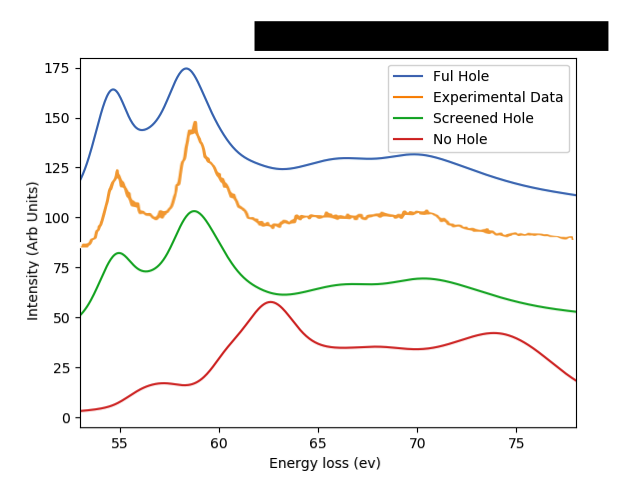
\includegraphics[scale=0.45]{Li2O_three}
	\caption{Lithium K edge of $ \mathrm{Li_2O} $ from the three calculations taken with varying degrees of core hole. }
	\label{Li2O_three}
\end{figure}

\section{Lithium}
Metallic lithium has previously presented a  number of challenges to experimental analysis. Theoretically, as a metal, it has been predicted to exhibit no core hole effects due to a large degree of valence screening. A density plot supports this notion, revealing that core  holes have a large impact on the electron density, see Fig \ref{Li_countours}.  The excited atom attracts a number of valence electrons and  distorts the electron clouds of the surrounding atoms more aggressively than in $ \mathrm{Li_2O} $.  Calculating the screening factor however reveals that the lithium core hole is in reality only $ \sim$41\% screened.  A comparison with experimental spectra confirms this fact, Fig \ref{Li_spectra}.


\begin{figure}
	\centering
	\includegraphics[scale=0.4]{Li_contours}
	\caption{Electron density map of metallic lithium, before (a) and after (b) introduction of a core hole on the starred atom.  The contours are on equal logarithmic scales.}
	\label{Li_countours}
\end{figure}




\begin{figure}
	\centering
	\begin{subfigure}{0.45\textwidth}
		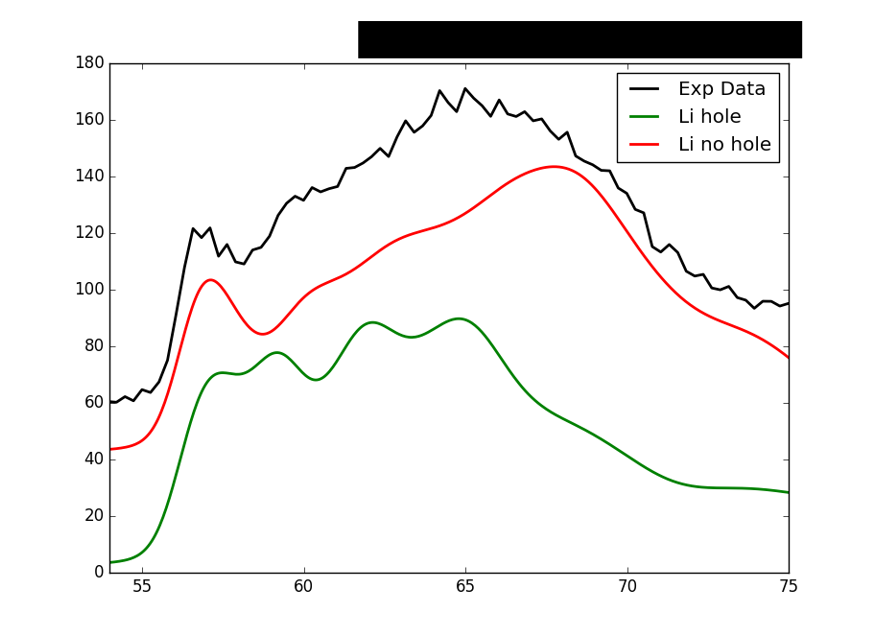
\includegraphics[scale=0.4]{Li_two}
	\end{subfigure}
	\hfill
	\begin{subfigure}{0.45\textwidth}
		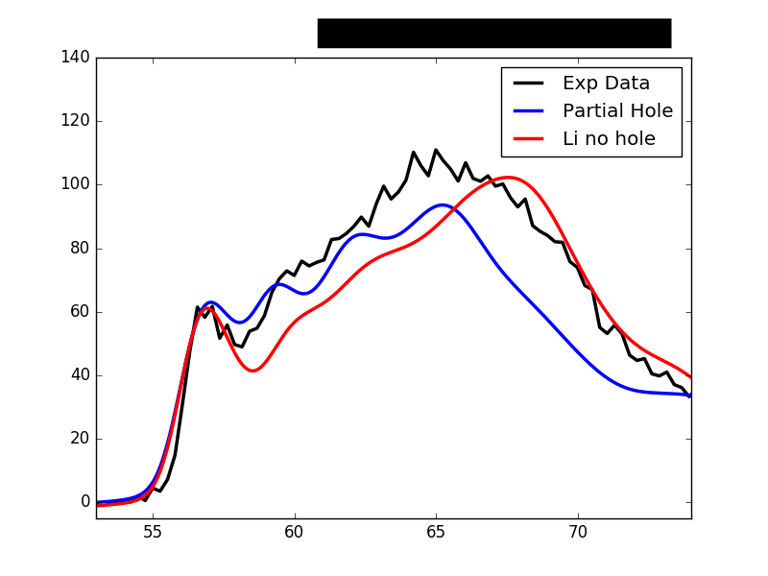
\includegraphics[scale=0.45]{Li_comparisson}
	\end{subfigure}

	\caption{Lithium K edge of Li from the three calculations taken with varying degrees of core hole. On the left, the full and no hole results are presented, on the right the screened hole spectrum is compared to the no hole spectrum, both normalized to the experimental result at 56 eV }
	\label{Li_spectra}
\end{figure}


Again, the literature predicts the superior agreement between full hole and no hole, but both are inferior to the screened hole result.  Of particular note is the small peak located at $ \sim$58 eV, which is underestimated, in the no hole spectra, overestimated in the full hole, and correctly accounted for in the screened case.  The only moderate (41\%) screening goes against common convention in the literature that metals do not exhibit core hole effects.  A couple of more extreme cases have been highlighted  (Cu, Al?), but the significant improvements observed with lithium suggest that screened core holes should be included or at least calculated in all cases.  It should be noted that lithium's lack of core electron screening may also contribute to the large core hole effects, which could be lessened for heavier elements. 

\section{LiF}
LiF has been one of the more published EELS results for lithium and simulations have obtained good agreement with a full core hole approximation \cite{mauchamp_ab_2006}.  A qualitative probe of the electron density after introducing a core hole reveals lesser effects than in Li and $ \mathrm{Li_2O} $ , see Fig \ref{LiF_countours}.  We can see that the introduction of a hole has minor effects on the electron density, but these are largely limited to slight distortions in the fluorine electron cloud. Additionally, despite the loss of a core electron, the density around the excited lithium atom retains much of its initial form. The minimal effect of introducing a core hole is reflective of fluorine's high electronegativity which ``freezes" all of the electrons in place and minimizes valence electron screening.  This effect is confirmed by calculating the screening coefficient which was determined to be zero in this case. Consequently, LiF represents the no screening case of Eqn. \ref{density_calc} and we can take the full hole spectra as the final spectrum.  Plotting the spectra against experiment confirms that a full hole does indeed produce good agreement, Fig \ref{LiF_spectra}.  The lack of screening in LiF also explains the good results obtained in literature when using only a full hole.  It also supports the theory that inserting a full hole is sufficient in the case of strong insulators, although again, lithium's lack of core screening limit may be contributing to this result.

\begin{figure}
	\centering
	\includegraphics[scale=0.35]{LiF_countours}
	\caption{Electron density map of LiF, before (a) and after (b) introduction of a core hole on the starred atom.  The contours are on equal logarithmic scales.}
	\label{LiF_countours}
\end{figure}

\begin{figure}
	\centering
	\includegraphics[scale=0.45]{LiF_colour}
	\caption{Lithium K edge of LiF from the two calculations taken with varying degrees of core hole. }
	\label{LiF_spectra}
\end{figure}



\section{Li-LiF Mixture}
The full importance of including screening in core hole calculations is demonstrated when investigating a mixed phase crystal.  When obtaining the spectra for LiF, a transformation to metallic lithium is observed, due to the beam damage.   During this transformation, acquired intermediate spectra display elements from both LiF and Li.  To investigate the transformation, a linear combination of the spectra from metallic lithium and LiF was compared to the experimental result, see Fig \ref{mix-screened}.  The good agreement obtained here supports both the inclusion of screening and that the sample contains  Li, LiF, and no intermediate phases or contamination.  The importance of screening is highlighted in Fig \ref{mix-unscreened}, where the no hole lithium spectra is used, resulting in a poorer fit, that fails to reproduce the peak at 59eV.  This unaccounted for peak would prevent such an  analysis from confirming the purity of the sample and of the mixture.  



\begin{figure}
	\centering
	\begin{subfigure}{0.45\textwidth}
		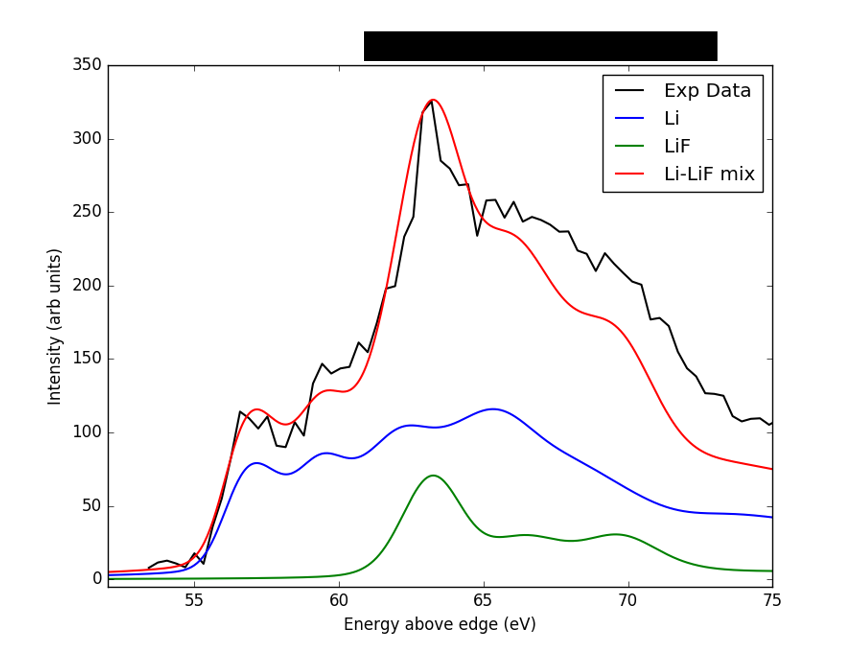
\includegraphics[scale=0.4]{Li-Lif_colour}
		\caption{}
		\label{mix-screened}
	\end{subfigure}
\hfill
	\begin{subfigure}{0.45\textwidth}
		\includegraphics[scale=0.5]{Li-LiF_mix_no-screen}
		\caption{}
		\label{mix-unscreened}
	\end{subfigure}
	\caption{Lithium K edge of Li-LiF mix using full hole LiF spectrum and screened (a) and unscreened (b) Li spectrum. }

\label{Li-LiF_mix_screened}
\end{figure}



\section{Discussion}
The cases handled here highlight the importance of including a core hole and calculating screening effects when performing ELNES on lithium.  In every case, a core hole was necessary, including metallic lithium which has been predicted to not exhibit core hole effects.  Additionally, in every case except LiF, screening is non negligible and the first order method developed in Chapter \ref{methods} results in dramatic improvements to experimental agreement.  The impact of including screening in ELNES calculations is made more apparent when dealing with unknown cases such as the Li-LiF mixture where it is essential to fingerprinting the near edge structure.  The improvement to the peak ratio in $ \mathrm{Li2O} $ is another key feature in terms of identifying oxidation on lithium edges, or taking the steps to quantitative analysis.  Finally the reliable agreement between calculation and experiment help solidify the validity of the technique of performing EELS at 30keV to analyze beam sensitive materials, a result with considerably less weight without excellent agreement between the results.  






\chapter{Conclusion}\label{conclusion}

The main objectives of this work have been to develop a better means to simulate EELS spectra in the context of lithium materials and further verify the reliability of EELS at 30 keV.  The first order screening method presented in Chapter \ref{methods} is a step in the right direction.  It represents a dramatic improvement to the current methods and results in superior agreement between simulation and experiment in every case treated in this work.  Most importantly, the method achieves these improvements without requiring  empirical data or \textit{ad hoc} assumptions and maintains the computational scaling rate of previous methods. Ensuring that the method relies only on first principles enables it to reveal unintuitive results such as the unscreened hole in metallic lithium, and predict unknown systems such as the metallic lithium-lithium fluoride compound.  The success of the method at matching the experimental 30 keV EELS is a strong argument for both the validity and potential of low energy EELS as a tool to analyze beam sensitive materials.  \\

However, there is still considerable room for improvement in EELS calculations.  Experimental equipment and techniques continue to advance to study more intricate materials. The screening calculations in this work were tailored to lithium's various peculiarities and restricted to crystalline materials.  The improvements for lithium materials highlight the need for more general methods to support all elements, as well as amorphous and non infinite samples.  Additionally, the majority of theoretical EELS analysis remains qualitative and the realm of quantitative EELS presents an entirely new set of challenges. The ultimate goal of entirely predictive methods capable of performing quantitative analysis on any material remains out of reach and presents a target for future efforts. \\


 





\end{document}